\documentclass[11pt]{article}
%\renewcommand{\thesection}{\Roman{section}}  %zmiana section na rzymskie
\usepackage[utf8]{inputenc}
\usepackage[OT4]{polski}
\usepackage{tabularx}
\usepackage[margin=60pt]{geometry}
\usepackage{amsmath}
\usepackage{amsfonts}
\usepackage{listings} 
\usepackage[usenames,dvipsnames,table,xcdraw]{xcolor}
\usepackage{array}
\usepackage{sidecap} %do grafik
\usepackage{wrapfig} % j. w.
\usepackage{graphicx} %j.. w.
\usepackage{subfig} %j. w.
\usepackage{booktabs}
\usepackage{longtable}
\usepackage{hyperref}
\usepackage{nicefrac}
\usepackage{multirow}

\begin{document}
%%%%%%%%%%%%%%%%%%%%%%%%%%%%%%%%%%%%%%%%%%%%%%%%%%%%%%%%%%%%%%%%%%%%%%%%%%%%%%%
%%	tabelka
%%%%%%%%%%%%%%%%%%%%%%%%%%%%%%%%%%%%%%%%%%%%%%%%%%%%%%%%%%%%%%%%%%%%%%%%%%%%%%%%

\begin{table}[h!]
	\begin{tabular}{|l|l|l|l|l|l|}	\hline
	\textbf{Laboratorium} & \multirow{2}{*}{ \textbf{\LARGE 1} } & \multicolumn{3}{l|}{ \textbf{Spektroskopia fluorescencji} } &
	\multirow{3}*{\begin{tabular}{l} Zespół w składzie: \\ 1. Paweł Rzońca \\ 2. Paweł Kozioł \\ 3. Agata Sławska\end{tabular}  }\\
	\textbf{Fizyki Ciała Stałego} & & \multicolumn{3}{l|}{\textbf{rentgenowskiej (XRF)}} &\\
	\cline{1-5}
	Wydział: \textbf{WFiIS} & \multicolumn{3}{l|}{Kierunek: \textbf{Fizyka Techniczna}} & \multicolumn{1}{p{2cm}|}{Rok: \textbf{3}} & \\
	\cline{1-5}
	\multicolumn{3}{|l|}{Data wykonania: \textbf{19.11.2015} } & Data oddania: \textbf{3.12.2015} &\multicolumn{1}{l|}{ Ocena:} &\\
	\hline
	\end{tabular}
\end{table}

%%%%%%%%%%%%%%%%%%%%%%%%%%%%%%%%%%%%%%%%%%%%%%%%%%%%%%%%%%%%%%%%%%%%%%%%%%%%%%%%


\section*{Aparatura i metodyka}
\begin{itemize}
\item 
\item 
\item 
\end{itemize}

%%%%%%%%%%%%%%%%%%%%%%%%%%%%%%%%%%%%%%%%%%%%%%%%%%%%%%%%%%%%%%%%%%%%%%%%%%%%%%

\section*{Opracowanie wyników}

\subsection*{Próbka pierwsza - moneta}

Na wykresie \ref{wykres_1} zamieszczono widmo promieniowania uzyskane po wykonaniu pomiarów i oznaczeniu pasujących pików pierwiastków Cu i Ni z podziałem na linie $K_{\alpha}, K_{\beta}$.\\

\begin{figure}[h!] %% [h!] mówi kompilatorowi, że bardzo chcemy aby ten obrazek był dokładnie tu
\begin{center}
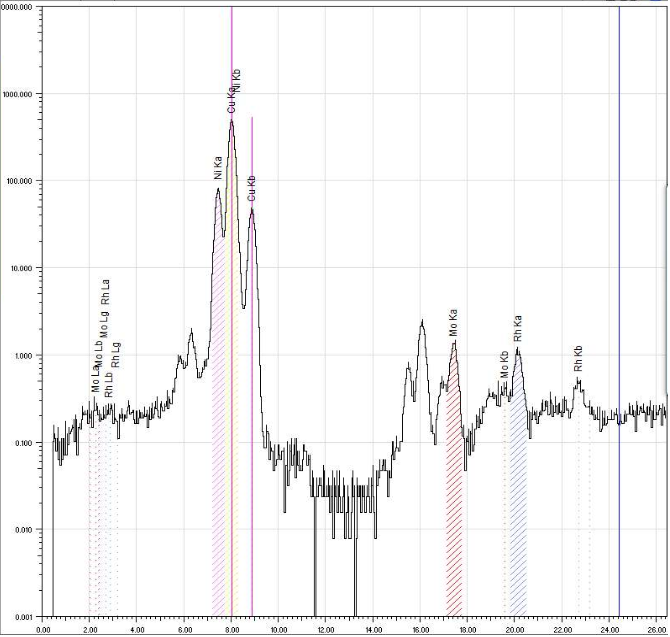
\includegraphics[scale=0.6]{moneta1.png}
\caption{Widmo promieniowania fluorescencyjnego dla monety.}
\label{wykres_1}
\end{center}
\end{figure}

Następnym krokiem było przeprowadzenie analizy mającej na celu wyznaczenie udziału procentowego poszczególnych pierwiastków. 
Otrzymane wyniki zamieszczono w \ref{tab_1}\\
\\	
\begin{table}[h!]
\begin{center}
\caption{Skład pierwiastkowy próbki pierwszej.}\label{tab_1}
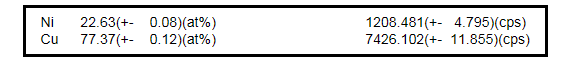
\includegraphics[scale=0.8]{moneta_il.png}\\
\end{center}
\end{table}

Na podstawie składu procentowego zauważono dominujący udział miedzi do zawartości niklu w stosunku 77$\div$23\%.\\

%%%%%%%%%%%%%%%%%%%%%%%%%%%%%%%%%%%%%%%%%%%%%%%%%%%%%%%%%%%%%%%%%%%%%%%%%%%%%%%

\subsection*{Próbka druga - kamień}  

Kolejną próbką, którą poddano analizie był kamień. Na wykresie \ref{wykres_2} przedstawiono widmo promieniowania drugiej próbki otrzymane po wykonaniu pomiarów i oznaczeniu pasujących do pików pierwiastków Fe, Ti, W, Nb i Mo z podziałem na linie $K_{\alpha}, K_{\beta}$.\\
\begin{figure}[h!]
\begin{center}
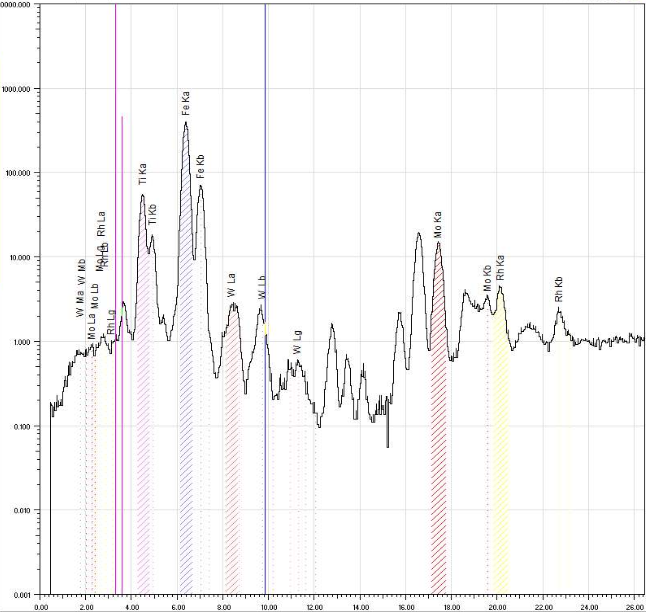
\includegraphics[scale=0.6]{kamyk_biale.png}\\
\caption{Widmo promieniowania fluorescencyjnego dla kamienia.}
\label{wykres_2}
\end{center}
\end{figure}

Po zidentyfikowaniu występujących pierwiastków przystąpiono do analizy ilościowej danej próbki. Otrzymane wyniki zamieszczono w tabeli \ref{tab_2}.\\
\\	
\begin{table}[h!]
\begin{center}
\caption{Skład pierwiastkowy próbki drugiej.}\label{tab_2}
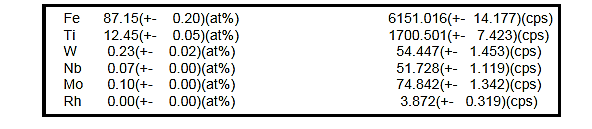
\includegraphics[scale=0.8]{kamyk_biale_il.png}\\
\end{center}	
\end{table}

Na podstawie składu procentowego stwierdzono, że badany kamień składa się głównie z  żelaza,\\
bo aż z 87\% i tytanu 12\% oraz śladowych ilości takich pierwiastków jak wolfram czy niob, 
oznaczony molibden i rod pochodzą od przesłony oraz anody lampy rentgenowskiej.\\

%%%%%%%%%%%%%%%%%%%%%%%%%%%%%%%%%%%%%%%%%%%%%%%%%%%%%%%%%%%%%%%%%%%%%%%%%%%%%%%
	
\subsection{Próbka trzecia - złoty łańcuszek}

Ostatnią próbką, dla której przeprowadzono analizę był złoty łańcuszek. Na wykresie \ref{wykres_3} przedstawiono widmo promieniowania drugiej próbki otrzymane po wykonaniu pomiarów i oznaczeniu pasujących do pików pierwiastków Au i Cu z podziałem na linie $K_{\alpha}, K_{\beta}$.\\

\begin{figure}[h!]
\centering %% to samo co \begin{center} ... \end{center} dla całego otoczenia figure. to samo w table
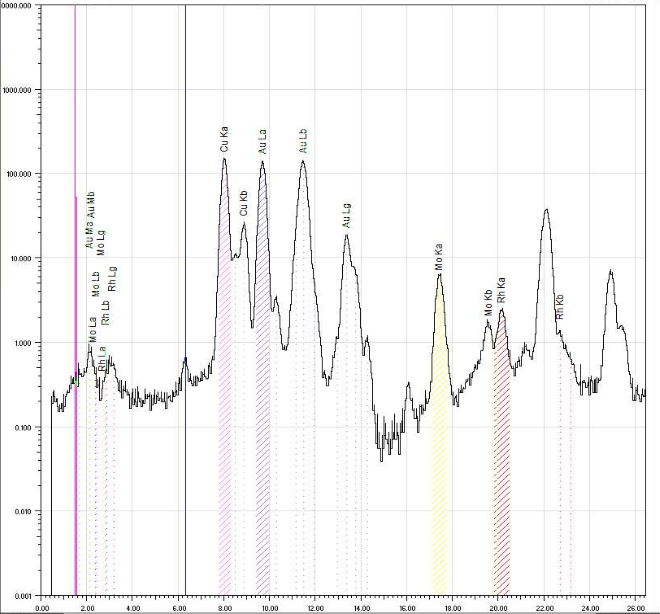
\includegraphics[scale=0.6]{lancuszek.png}
\caption{Widmo promieniowania fluorescencyjnego dla złotego łańcuszka.}
\label{wykres_3}
\end{figure}

Następnie dla danej próbki przeprowadziliśmy kolejną analizę mającą na celu wyznaczenie udziału procentowego poszczególnych pierwiastków. Otrzymane wyniki zamieszczono w tabeli \ref{tab_3}.\\
\\	
\begin{table}[h!]
\centering
\caption{Skład pierwiastkowy próbki trzeciej.}\label{tab_3}
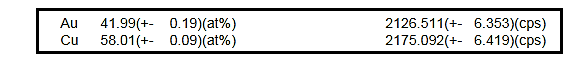
\includegraphics[scale=0.8]{lancuszek_il.png}\\
\end{table}

Na podstawie otrzymanych wyników zauważono, że badany przez nas łańcuszek składa się z 58\% miedzi i 42\% złota.\\

%%%%%%%%%%%%%%%%%%%%%%%%%%%%%%%%%%%%%%%%%%%%%%%%%%%%%%%%%%%%%%%%%%%%%%%%%%%%%%
	
\section*{Wnioski}

Podczas oznaczania jakościowego największym wyzwaniem było odnalezienie odpowiednich pierwiastków oraz odrzucenie
wzbudzeń dwufotonowych, wyraźnie odznaczające się w przypadku dwóch pierwszych próbek.  
W tabelach \ref{tab_1}, \ref{tab_2} oraz \ref{tab_3} zebrano wyniki pomiarów ilościowych składu pierwiastków w badanych próbkach. 
Badaną monetą była 50-centówka brytyjska, którą wytwarza się ze stopu miedzi i niklu w proporcjach 3/1. Otrzymany wynik jest jak najbardziej sensowny.
W drugiej próbce podejrzewano znaleźć wolfram jednak badanie wykazało wyłącznie jego ilości śladowe.
W złotym łańcuszku, tak jak przypuszczano, oznaczono złoto oraz miedź. 
\end{document}


